%===============================================================================

\documentclass[conference]{IEEEtran}
% Include all packages from file.
% Report template for Mälardalen University
% Original template can be found: 
% https://www.overleaf.com/latex/templates/ieee-bare-demo-template-for-conferences/ypypvwjmvtdf
% Template file structure organised by: Emil Persson
% The following packages should follow the IEEE conference guidelines.

%===============================================================================
% QoL

%===============================================================================
% Add packages here

\usepackage{comment}
\usepackage[nolist,nohyperlinks]{acronym}
\usepackage{datetime}
\usepackage{amsmath}
\usepackage{cuted}
\usepackage{pdfpages}

% Tables
\usepackage{tabularx}
\usepackage{longtable}
\usepackage[table,xcdraw]{xcolor}

%===============================================================================
%===============================================================================
% Define acronyms here

\acrodef{stad}[STAD]{Safe Trustworthy Autonomous Deliverance System}

% Universities
\acrodef{udea}[UdeA]{Universidad de Antioquia}
\acrodef{utp}[UTP]{Universidad Tecnológica de Panamá}
\acrodef{mdu}[MDU]{Mälardalens Universitet}

% Management
\acrodef{wbs}[WBS]{Work Breakdown Structure}
\acrodef{bom}[BOM]{Bill of Materials}

% Software
\acrodef{ai}[AI]{Artificial Intelligence}
\acrodef{api}[API]{Application Programming Interface}
\acrodef{ros2}[ROS2]{Robot Operating System 2}
\acrodef{hil}[HIL]{Hardware-in-the-Loop}
\acrodef{mappo}[MAPPO]{Multi-Agent Proximal Policy Optimization}
\acrodef{udp}[UDP]{User Datagram Protocol}
\acrodef{ppo}[PPO]{Proximal Policy Optimization}
\acrodef{foc}[FOC]{Field-Oriented Control}
\acrodef{ros}[ROS]{Robot Operating System}
\acrodef{gui}[GUI]{Graphical User Interface}
\acrodef{slam}[SLAM]{Simultaneous Localization And Mapping}
\acrodef{micro-ros}[micro-ROS]{mirco-Robot Operating System}
\acrodef{fifo}[FIFO]{First In, First Out}
\acrodef{rgb}[RGB]{Red, Green, and Blue}
\acrodef{rf}[RF]{Radio Frequency}
\acrodef{rl}[RL]{Reinforcement Learning}
\acrodef{os}[OS]{Operating System}

% Hardware
\acrodef{cad}[CAD]{Computer-aided Design}
\acrodef{ic}[IC]{Integrated Circuit}
\acrodef{imu}[IMU]{Inertial Measurement Unit}
\acrodef{pcb}[PCB]{Printed Circuit Board}
\acrodef{mcu}[MCU]{Micro Controller Unit}
\acrodef{lidar}[LIDAR]{Light Detection and Ranging}
\acrodef{cpu}[CPU]{Central Processing Unit}
\acrodef{spi}[SPI]{Serial Peripheral Interface}
\acrodef{esc}[ESC]{Electronic Speed Controller}
\acrodef{i2c}[I$^2$C]{Inter-Integrated Circuit}
\acrodef{uart}[UART]{Universal Asynchronous Receiver-Transmitter}
\acrodef{pc}[PC]{Personal Computer}
\acrodef{gpio}[GPIO]{General-Purpose Input/Output}
\acrodef{pwm}[PWM]{Pulse-Width Modulation}
\acrodef{rpm}[RPM]{Revolutions Per Minute}
\acrodef{led}[LED]{Light-Emitting Diode}
\acrodef{dof}[DoF]{Degrees of Freedom}
\acrodef{hal}[HAL]{Hardware Abstraction Layer}
\acrodef{hdmi}[HDMI]{High-Definition Multimedia Interface}

% Physics
\acrodef{v}[V]{Voltage}

% SSL
\acrodef{ssl}[SSL]{Small Size League}

%===============================================================================
%===============================================================================
% Do definitions here

%-------------------------------------------------------------------------------

\definecolor{na}{RGB}{130, 130, 130} % Gray for N/A

\definecolor{c}{RGB}{255, 100, 100} % Red for Canceled

\definecolor{h}{RGB}{255, 255, 0} % Yellow for On Hold

\definecolor{p}{RGB}{255, 165, 0} % Orange for progress

\definecolor{d}{RGB}{90, 255, 90}  % Green for completed (done)

\definecolor{u}{RGB}{70, 130, 255} % Blue for upcoming

%===============================================================================

%===============================================================================
% Template stuff

% Swedish language package 
\usepackage[utf8]{inputenc}
\usepackage[T1]{fontenc}
\usepackage[swedish,english]{babel}

% Graphics
\usepackage{graphicx, float, subfigure, blindtext}

\newcommand\IEEEhyperrefsetup{
bookmarks=true,bookmarksnumbered=true,%
colorlinks=true,linkcolor={black},citecolor={black},urlcolor={black}%
}

% Preferred hyperref setup, Michael Shell
\usepackage[\IEEEhyperrefsetup, pdftex]{hyperref}

% Maths
\usepackage{mathtools}

% These packages must be at the end
\usepackage{cleveref}
\graphicspath{{images/}}

% Remove section first paragraph indent
\usepackage{titlesec}
\titlespacing*{\section}{0pt}{*1}{*1}
\titlespacing*{\subsection}{0pt}{*1}{*1}
\renewcommand{\thesubsubsection}{\arabic{subsubsection}}
\titleformat{\subsubsection}[runin]{\itshape}{\thesubsubsection)}{1em}{}[:]
\titlespacing*{\subsubsection}{\parindent}{0pt}{*1}

%===============================================================================
% Author

% Include authors 
\author{\IEEEauthorblockN{ %
Viktor Eriksson\IEEEauthorrefmark{1},
Anton Grusell\IEEEauthorrefmark{2}, 
Mudar Ibrahim\IEEEauthorrefmark{3},
Jacob Johanssson\IEEEauthorrefmark{4},
Aaiza Aziz Khan\IEEEauthorrefmark{5},
Carl Larsson\IEEEauthorrefmark{6},\\
Johanna Melander\IEEEauthorrefmark{7},
Shruti Puthiya Kunnon\IEEEauthorrefmark{8},
Pontus Svensson\IEEEauthorrefmark{9},
Fredrik Westerbom\IEEEauthorrefmark{10},
Emil Åberg\IEEEauthorrefmark{11}
}
\IEEEauthorblockA{
School of Innovation, Design and Engineering, M.Sc.Eng Robotics\\
Mälardalens University, Västerås, Sweden\\
Email:
\{\IEEEauthorrefmark{1}Ven20002, 
\IEEEauthorrefmark{2}agl19003,
\IEEEauthorrefmark{3}mim20004,
\IEEEauthorrefmark{4}jjn20030,
\IEEEauthorrefmark{5}akn23018,
\IEEEauthorrefmark{6}cln20001,\\
\IEEEauthorrefmark{7}Jmr19002,
\IEEEauthorrefmark{8}spn23001,
\IEEEauthorrefmark{9}psn19003,
\IEEEauthorrefmark{10}fnl18001, 
\IEEEauthorrefmark{11}eag24002\}@student.mdu.se
}}

%===============================================================================
% Title

% The report title.
\title{Multi-robot Soccer - RoboCup - PRO3\\
Mälardalen University}
% Document begins here
\begin{document}

%===============================================================================
% Commands needs to be included here for commands to work in document

%===============================================================================
% Define commands here

% dd-mm-yyyy format
% with zero padding to two digits for month and day
\makeatletter
\renewcommand{\today}{\the\year-\two@digits{\the\month}-\two@digits{\the\day}}
\makeatother

%===============================================================================

%===============================================================================
% Header stuff

% Create the title.
\maketitle
% Create date
\begin{strip}
    \begin{center}
        \today
    \end{center}
\end{strip}

%===============================================================================
% Sections

% Example sections, name them
% according to specific needs.
%===============================================================================
\section{Project Information}

% Project name
This paper covers the progress report for the project Multi-robot Soccer - RoboCup for the time period from 8th of November to 6th of December. 
% Collaboration
It is a collaboration project between \ac{mdu}, \ac{udea} and \ac{utp}. 
% Summary of project 
The project is about creating a \ac{ssl}-RoboCup robot and developing the accompanying software.
It is assumed that the reader is familiar with the project, for those who are not, see the project plan available in Appendix\:\ref{appendix}.
% Project members, their roles and their tasks
Table.\:\ref{tab:contributors_roles} outlines the team members, their roles, and their assigned tasks.
\begin{table}[H]
    \centering
    \caption{Project members, including their roles and assigned tasks.}
    \label{tab:contributors_roles}
    \begin{tabularx}{\columnwidth}{|X|X|X|} \hline
         \textbf{Name}          & \textbf{Role}                                         & \textbf{Task}                                 \\ \hline
         Viktor Eriksson        & Software developer                                    & Collective robot behaviour                    \\ \hline
         Anton Grusell          & Hardware developer                                    & 3D-\acs{cad} \& Body design                   \\ \hline
         Mudar Ibrahim          & Team leader \& Software developer                     & Communication                                 \\ \hline
         Jacob Johanssson       & Software developer                                    & Collective robot behaviour                    \\ \hline
         Aaiza Aziz Khan        & Software developer                                    & Communication                                 \\ \hline
         Carl Larsson           & Software lead \& Software developer                   & Individual robot behaviour \& Communication   \\ \hline
         Johanna Melander       & Hardware developer                                    & Mechanical design                             \\ \hline
         Shruthi Puthiya Kunnon & Software developer                                    & Communication                                 \\ \hline
         Pontus Svensson        & Team leader \& Hardware lead \& Hardware developer    & Power-train \& Electronics                    \\ \hline
         Fredrik Westerbom      & Hardware developer \& Software developer              & Sensors \& Hardware communication             \\ \hline
         Emil Åberg             & Software developer                                    & Communication                                 \\ \hline
    \end{tabularx}
\end{table}

%===============================================================================
%===============================================================================
\section{Project Progress Summary}

% !!! Reference back to the project plan !!!

% Provides a concise and informative summary of what has been achieved so far.
% Provide a high-level overview of the project's current status. Briefly mention problematic or delayed work packages, issues, or blockers that require stakeholder attention.


% TEAM LEADER will write this section!! No one is allowed to write here. 


% Overview of work package status 
As of \today, 3 out of 17 work packages have been completed, 9 are in progress\footnote{In progress also entails packages where a sizeable part of the work has been completed, but other parts have been cancelled.}, 0 have not started yet (upcoming), 0 are on hold and 5 have been cancelled. 
% Issues
The project has encountered substantial issues. Amongst the most notable are: components being delivered late or not being delivered at all; problems with software tools and the lack of documentation for the software tools; and the severe lack of time given the scope. All of this has caused most of the progress to fall short of fully achieving the milestones.
% State
The system as a whole is in an unfinished state, but some parts are in an operational state. Evaluating the systems performance against any metrics is not currently feasible. $90\%$ of the allocated budget for the project has been utilized, and the project will be unable to deliver according to the initial plan and requirements.

% What should be prioritized in future
Going forward with the project, it is strongly recommended that focus be placed on: 1.4 \textit{Communication protocol}, the individual parts can not be integrated without this crucial work package; and 1.3.2.3 \textit{Implement a velocity distributor}, to enable the robots to take velocity commands and output \ac{rpm} commands to each individual wheel motor.
% Advice
Furthermore, it is not advised to use STM32CubeIDE and the associated tool MC Workbench because of the buggy and unreliable state that they are in, as well as the poor error messages; nor the PyTorch C++ library because of its lack of documentation.

%===============================================================================

\begin{comment}

\end{comment}

%===============================================================================
%===============================================================================
\section{Work Package Status}

% !!! Reference back to the project plan !!!

% !!! ONLY WORK PACKAGES SHOULD BE COVERED !!!

All information regarding the work packages which are apart of the 8th of November to 6th of December work period are covered in the following subsections. Note that only work packages are covered, and that sub-work packages exist.

%-----------------------------------------------
% Description of columns:

% ID: ID of task/workpackage/deliverable.

% Name: Name of task/workpackage/deliverable.

% Planning status: "On-track" or "Off-track".

% Completion status:  "Not started", "On Hold", "Cancelled", "In Progress", or "Completed".

% Accountability: People responsible for the package.

% Recovery plan: If a package is "Off-track" then here you write the plan to get it back "On-track".

% Progress: Summary of progress, highlighting key outcomes and which tasks/deliverables have been completed. Include both ID and name of tasks and deliverables.

% Issues: List challenges/issues.

% Next steps: Outline the work package's next set of tasks or milestones. List the next deliverables and task which will be done, their ID and name.
%-----------------------------------------------

%-------------------------------------------------------------------------------

%-------------------------------------------------------------------------------

\subsection*{1.3 Hardware interface}
\begin{itemize}
    \item \textbf{Planning status}: Off-track
    \item \textbf{Completion status}: In Progress 
    \item \textbf{Accountability}: Mudar Ibrahim, Aaiza Aziz Khan, Carl Larsson, Shruthi Puthiya Kunnon, Fredrik Westerbom, Emil Åberg
    \item \textbf{Recovery plan}: Allocating additional work force. 
    \item \textbf{Progress}: 1.3.2 \textit{Wheel motor interface} is currently being worked on, with current efforts focused on task 1.3.2.1 \textit{Establish communication using \acs{uart}}, and 1.3.2.2 \textit{Implement \acs{foc}} having been completed. 
    
    Integrating \ac{micro-ros} for the purpose of setting up \ac{ros} subscriptions over \ac{uart} between Nucleo 144 and Raspberry PI (1.3.7) is currently being worked on. 1.3.5 \textit{Sensor interface} has been completed for all sensors that have not been cancelled (due to a lack of time or lack of hardware).
    \item \textbf{Issues}: The software used for testing the motors and developing the motor control algorithm (\ac{foc}), called MC Workbench 6 with the tool \acs{foc} Wizard, has proven problematic (Delft Mercurians also encountered problems with this software). This has resulted in an unexpected amount of time being spent on solving 1.3.2.
    
    The software tool STM32CubeIDE has also proven to be difficult to work with, not only because its poor debugging tool, but also because of issues with the generated code. From debugging Carl and Fredrik can determine that the \ac{esc} can receive \ac{rpm} values via \ac{uart}. However, the values seem to be inaccurate and are not updated continuously.
    %To mitigate these problems regarding task 1.3.2.1, Carl and Fredrik aim to test different baud rates, enable \ac{fifo} as well as debugging using the configurable red \ac{led} on the \ac{esc}.
    \item \textbf{Next steps}: N/A
\end{itemize}

%-------------------------------------------------------------------------------

\subsection*{1.3.5 Sensor interface}
\begin{itemize}
    \item \textbf{Planning status}: Off-track
    \item \textbf{Completion status}: In Progress
    \item \textbf{Accountability}: Mudar Ibrahim, Aaiza Aziz Khan, Shruthi Puthiya Kunnon, Emil Åberg
    \item \textbf{Recovery plan}: Accept that the robot will be without wheel encoders, camera and break bream.
    \item \textbf{Progress}: Implementation of device drivers which allows the reading of \ac{imu}, \ac{lidar} and \ac{rgb} sensor measurements on STM32 via \ac{i2c} has been completed (1.3.5.1.2, 1.3.5.4.1, 1.3.5.5.1). 1.3.5.2 \textit{Wheel encoders} can not be implemented since the wheel encoders have yet to be delivered, hence it was cancelled. 1.3.5.3 \textit{Camera} was cancelled because of lack of time. 1.3.5.6 \textit{Break beam} was cancelled due to the project not being allowed to choose sensors freely.
    \item \textbf{Issues}: All device drivers for the sensors are full of \ac{hal} calls which can only execute on the STM32 microcontroller. This means it is not possible to write GoogleTest test cases which are to run on a PC. Also, STM32CubeIDE has its own project structure, separate from the one which is otherwise used throughout this project. A way to change it while keeping the functionality of the code generator intact was not found. It was decided that the project structure of STM32CubeIDE was to be used for the repository containing the STM32 software while keeping code that has been written by the project members (and not produced by the code generator) in a separate directory where all standards of the project are followed.
    \item \textbf{Next steps}: N/A
\end{itemize}

%-------------------------------------------------------------------------------

\subsection*{1.4 Communication protocol}
\begin{itemize}
    \item \textbf{Planning status}: On-track
    \item \textbf{Completion status}: Cancelled
    \item \textbf{Accountability}: Aaiza Aziz Khan, Shruthi Puthiya Kunnon, Emil Åberg
    \item \textbf{Recovery plan}: Theoretically, communication between Raspberry Pi and central computer should be able to be established using existing hardware together with \ac{ros}, which has built-in support for Wi-Fi communication. However, every developer who has \ac{ros} familiarity is currently busy with other work.
    \item \textbf{Progress}: None
    \item \textbf{Issues}: Development of custom \ac{rf} communication has been cancelled due to lack of time.
    \item \textbf{Next steps}: N/A
\end{itemize}

%-------------------------------------------------------------------------------

\subsection*{1.5 Individual robot behaviour}
\begin{itemize}
    \item \textbf{Planning status}: Off-track
    \item \textbf{Completion status}: In Progress
    \item \textbf{Accountability}: Carl Larsson
    \item \textbf{Recovery plan}: It was deemed unrealistic to find the solution for the nav2 configuration problem (1.5.5 \textit{nav2 stack configuration}) according to Carl Larsson and Pontus Svensson (the most experienced \ac{ros2} developers on the team). The compromise instead became running with \ac{slam} since the nav2 stack and the developed code worked as intended when doing so. This was a sacrifice which increased the computational demands of the Raspberry Pi executable, but it ensures additional time is not wasted debugging after having debugged for 4 weeks already, leaving a more optimal solution for future work. With this new approach, 1.5.5 \textit{nav2 stack configuration} will be considered complete.
    \item \textbf{Progress}: The base functionality is complete. 1.5.6 \textit{Develop supporting functions} remains, having its activities cancelled due to 1.4 \textit{Communication protocol} and some miscommunications. 1.5.7 \textit{Computer vision} was also cancelled since it was discovered late in the project when it was no longer possible to develop it.
    \item \textbf{Issues}: Problems with getting nav2 to work without using \ac{slam}. Other issues include: miscommunication, activity dependencies, time and work force constraints.
    \item \textbf{Next steps}: N/A
\end{itemize}

%-------------------------------------------------------------------------------

\subsection*{1.5.6 Develop supporting functions}
\begin{itemize}
    \item \textbf{Planning status}: Off-track
    \item \textbf{Completion status}: Cancelled
    \item \textbf{Accountability}: Carl Larsson
    \item \textbf{Recovery plan}: N/A
    \item \textbf{Progress}: Was waiting for 1.3 \textit{Hardware interface} to complete before being able to proceed with 1.5.6.1.2 \textit{Run and call on Hardware interface}. 1.5.6.1.1 \textit{Run and call on Simulation interface} was cancelled since this task would cause an overly complicated software structure. The simulation instead directly interfaces with 1.6 \textit{Collective robot behaviour}, this will act as a proof of concept for the \ac{ai} algorithms ability to learn. 1.5.6.2 \textit{Ability to send data}, 1.5.6.3 \textit{Ability to receive data} and 1.5.6.4 \textit{Initialize the robot} were cancelled since 1.4 was cancelled, and because there was some miscommunication regarding hardware initialisation of the robot, complicating the process of obtaining its ID, this is now left for future work.
    \item \textbf{Issues}: Heavy dependencies on other parts make development impossible until the other parts have been completed.
    \item \textbf{Next steps}: N/A
\end{itemize}

%-------------------------------------------------------------------------------

\subsection*{1.5.7 Computer vision}
\begin{itemize}
    \item \textbf{Planning status}: Unknown
    \item \textbf{Completion status}: Cancelled
    \item \textbf{Accountability}: N/A
    \item \textbf{Recovery plan}: N/A
    \item \textbf{Progress}: None
    \item \textbf{Issues}: Poor planning and oversights caused this package to not be discovered until it was too late to implement.
    \item \textbf{Next steps}: N/A
\end{itemize}

%-------------------------------------------------------------------------------

\subsection*{1.6 Collective robot behaviour}
\begin{itemize}
    \item \textbf{Planning status}: Off-track
    \item \textbf{Completion status}: In Progress
    \item \textbf{Accountability}: Viktor Eriksson, Jacob Johansson
    \item \textbf{Recovery plan}: Everything will be documented, and code will be restructured to be more simple and easy to follow for the next year's students. This will allow future work to continue working on implementing the algorithm.
    \item \textbf{Progress}: Found a way to speed up grSim, making it faster to train the algorithm. Deliverables 1.6.3 \textit{Be able to send data}, 1.6.4 \textit{Be able to receive data} and 1.6.5 \textit{Ability to switch playing half on demand} were cancelled due to time constraints. Deliverable 1.6.2 \textit{Develop \acs{ai} for strategy planning} is still in progress, current efforts are being put into debugging the code to understand why the algorithm is not learning. This is partially due to a misunderstanding of how the algorithm works, because it was explained ambiguously in its paper.
    \item \textbf{Issues}: The robots do not seem to learn the objectives. However, there are no performance metrics to prove this or provide some form of analysis, it is therefore important that this is implemented.
    \item \textbf{Next steps}: Implement performance metrics for the algorithm to simplify analysis.
\end{itemize}

%-------------------------------------------------------------------------------

\subsection*{2.1 Base design}
\begin{itemize}
    \item \textbf{Planning status}: Off-track
    \item \textbf{Completion status}: In Progress
    \item \textbf{Accountability}: Anton Grusell, Johanna Melander, Pontus Svensson, Fredrik Westerbom
    \item \textbf{Recovery plan}: Accept
    \item \textbf{Progress}: 2.1.3 \textit{3D-design} and 2.1.4 \textit{Circuit design and integration} are in progress, with a majority of their activities completed.
    \item \textbf{Issues}: 2.1.3.3 \textit{Dribbler design} had to be redesigned to fit another motor.
    \item \textbf{Next steps}: N/A 
\end{itemize}

%-------------------------------------------------------------------------------

\subsection*{2.1.3 3D-design}
\begin{itemize}
    \item \textbf{Planning status}: Off-track
    \item \textbf{Completion status}: In Progress
    \item \textbf{Accountability}: Anton Grusell, Johanna Melander, Pontus Svensson
    \item \textbf{Recovery plan}: Accept
    \item \textbf{Progress}: 2.1.3.1 \textit{Chassis design}, 2.1.3.2 \textit{Wheel design} and 2.1.3.4 \textit{Kicker assembly design} have been completed. 2.1.3.3 \textit{Dribbler design}  and 2.1.3.5 \textit{Mounting design} are in progress.
    \item \textbf{Issues}: Issues regarding size constraints remain. Due to the dribbler motor not being delivered, the dribbler design is being redesigned to hold a smaller motor.
    \item \textbf{Next steps}: N/A
\end{itemize}

%-------------------------------------------------------------------------------

\subsection*{2.1.4 Circuit design and integration}
\begin{itemize}
    \item \textbf{Planning status}: Off-track
    \item \textbf{Completion status}: In Progress
    \item \textbf{Accountability}: Anton Grusell, Johanna Melander, Pontus Svensson
    \item \textbf{Recovery plan}: Due to delays in 2.1.4.2 \textit{Design kicker circuit}, the integration of the kicker circuit with the mainboard \ac{pcb} has been excluded in this iteration of the project. However, it is possible to add the control circuitry for the kicker circuit to the mainboard but it will require additional development time. 
    \item \textbf{Progress}: All circuits have been integrated with the mainboard \ac{pcb} except 2.1.4.9 \textit{Design kicker \ac{pcb}} as it is dependent on 2.1.4.2 \textit{Design kicker circuit} and the \acp{pcb} could not wait any longer for 2.2 \textit{Manufacturing}.
    \item \textbf{Issues}: Control circuitry on 2.1.4.2 \textit{Design kicker circuit} has delayed the final design and integration of 2.1.4.4 \textit{Design microcontroller circuit} and 2.1.4.7 \textit{Design mainboard PCB}.
    \item \textbf{Next steps}: 2.2 \textit{Manufacturing}
\end{itemize}

%-------------------------------------------------------------------------------

\subsection*{2.2 Manufacturing}
\begin{itemize}
    \item \textbf{Planning status}: Off-track 
    \item \textbf{Completion status}: In Progress
    \item \textbf{Accountability}: Anton Grusell, Johanna Melander, Pontus Svensson
    \item \textbf{Recovery plan}: Accept
    \item \textbf{Progress}: 2.2.1.1 \textit{Mainboard}, 2.2.1.4 \textit{Motor driver carrier board} and 2.2.1.5 \textit{Encoder board} \acp{pcb} have all been manufactured and is awaiting the delivery of three components before being able to be completed. 2.2.2.1 \textit{Manufacture chassis} is in progress. 2.2.2.2 \textit{Manufacture wheels} is completed. 2.2.2.4 \textit{Manufacture kicker} is in progress. 2.2.2.5 \textit{Manufacture mountings} is in progress.
    \item \textbf{Issues}: 2.2.1.1 \textit{Mainboard} is waiting for the delivery of two components, power inductor and socket headers. 2.2.1.4 \textit{Motor driver carrier board} is waiting for the delivery of a socket header. 2.2.1.5 \textit{Encoder board} is waiting for the delivery of the encoder \ac{ic}.
    \item \textbf{Next steps}: 2.3 \textit{Testing}. 
\end{itemize}

%-------------------------------------------------------------------------------

\subsection*{2.3 Testing}
\begin{itemize}
    \item \textbf{Planning status}: Off-track
    \item \textbf{Completion status}: In Progress
    \item \textbf{Accountability}: Anton Grusell, Johanna Melander, Pontus Svensson, Fredrik Westerbom
    \item \textbf{Recovery plan}: Accept
    \item \textbf{Progress}: The testing is dependent on 2.1.4 \textit{Circuit design and integration}, 2.2 \textit{Manufacturing} and the delivery of all components. This has resulted in a majority of this work package being cancelled. However, the test phase for the kicker has begun (2.3.2 \textit{Test kicker}). 2.3.3 \textit{Test dribbler} is in progress in the mechanical testing phase.
    \item \textbf{Issues}: Delays in 2.1.4 \textit{Circuit design and integration}, 2.2 \textit{Manufacturing} and components not being delivered, has made it difficult to start with 2.3 \textit{Testing}.
    \item \textbf{Next steps}: N/A
\end{itemize}

%-------------------------------------------------------------------------------

\subsection*{3.1 Develop \acs{hil}}
\begin{itemize}
    \item \textbf{Planning status}: Unknown
    \item \textbf{Completion status}: Cancelled  
    \item \textbf{Accountability}: N/A
    \item \textbf{Recovery plan}: N/A
    \item \textbf{Progress}: None
    \item \textbf{Issues}: Time and resource constraints.
    \item \textbf{Next steps}: N/A
\end{itemize}

%-------------------------------------------------------------------------------

\subsection*{3.2 Validate hardware platform}
\begin{itemize}
    \item \textbf{Planning status}: Unknown
    \item \textbf{Completion status}: Cancelled 
    \item \textbf{Accountability}: N/A
    \item \textbf{Recovery plan}: N/A
    \item \textbf{Progress}: None
    \item \textbf{Issues}: Time and resource constraints.
    \item \textbf{Next steps}: N/A
\end{itemize}

%-------------------------------------------------------------------------------

%===============================================================================

\begin{comment}

\end{comment}

%===============================================================================
%===============================================================================
\section{Completed and Upcoming Activities}

% Milestones achieved
The project has achieved no milestones since the last progress report, milestones have only partially been reached.
% Completed and Upcoming Activities
The completed and the upcoming activities for the project are shown in Table.\:\ref{tab:activity_status}, which is the \ac{wbs} with the addition of a new column indicating the status of the activity.

\onecolumn
\begin{longtable}{|c|c|m{0.6\textwidth}|c|}
    % Caption and label
    \caption{Summary of completed and upcoming activities. Green for completed, orange for in progress, yellow for on hold, red for cancelled, blue for upcoming.} \label{tab:activity_status} \\
    \hline
    % Fix header
    \textbf{ID} & \textbf{Work Class} & \textbf{Name (Work entailed)} & \textbf{Status} \\ \hline
    \endfirsthead
    % Fix next page headers
    \multicolumn{4}{|c|}{\textit{Continued from previous page}} \\ \hline
    \textbf{ID} & \textbf{Work Class} & \textbf{Name (Work entailed)} & \textbf{Status} \\ \hline
    \endhead
    \hline
    \endfoot
    \hline
    \hline
    \endlastfoot
%-------------------------------------------------------------------------------
    \rowcolor{na} - & Root & Multi-robot Soccer - RoboCup & - \\ \hline
    %--------------------
    % Software
    %--------------------
    \rowcolor{p} 1 & Category & Software & In Progress \\ \hline
    \rowcolor{d} 1.1 & Work Package & Simulate 12 robots & Completed \\ \hline
    \rowcolor{d} 1.1.1 & Deliverable & Setup grSim & Completed \\ \hline
    \rowcolor{d} 1.1.1.1 & Task & Download grSim & Completed \\ \hline
    \rowcolor{d} 1.1.1.2 & Task & Run the simulation correctly & Completed \\ \hline
    \rowcolor{d} 1.1.2 & Work Package & Simulation interface (\acs{api}) & Completed \\ \hline
    \rowcolor{d} 1.1.2.1 & Deliverable & Integrate Protobuf & Completed \\ \hline
    \rowcolor{d} 1.1.2.2 & Deliverable & Move a single robot & Completed \\ \hline
    \rowcolor{d} 1.1.2.3 & Deliverable & Activate kicker on a single robot & Completed \\ \hline
    \rowcolor{d} 1.1.2.4 & Deliverable & Activate dribbler on a single robot & Completed \\ \hline
    \rowcolor{d} 1.1.2.5 & Deliverable & Execute any desired control over any chosen robot in grSim & Completed \\ \hline
    \rowcolor{d} 1.2 & Work Package & \acs{ssl} interface (\acs{api}) & Completed \\ \hline
    \rowcolor{d} 1.2.1 & Deliverable & Integrate ssl-vision & Completed \\ \hline
    \rowcolor{d} 1.2.1.1 & Task & Receive single package containing positional data & Completed \\ \hline
    \rowcolor{d} 1.2.1.2 & Task & Receive continuous positional data & Completed \\ \hline
    \rowcolor{d} 1.2.2 & Deliverable & Integrate ssl-game-controller (human referee and optional auto referee) & Completed \\ \hline
    \rowcolor{d} 1.2.2.1 & Task & Receive a single package containing referee commands/signals & Completed \\ \hline
    \rowcolor{d} 1.2.2.2 & Task & Receive continuous stream of referee commands/signals & Completed \\ \hline
    \rowcolor{d} 1.2.2.3 & Task & Integrate AutoReferee & Completed \\ \hline
    \rowcolor{d} 1.2.3 & Deliverable & Develop an automatic game controller (will be used when training the \acs{ai}) & Completed \\ \hline
    \rowcolor{d} 1.2.3.1 & Task & Research and obtain proper understanding of \acs{ssl}-rules & Completed \\ \hline
    \rowcolor{d} 1.2.3.2 & Task & Implement the automatic game controller system & Completed \\ \hline
    \rowcolor{p} 1.3 & Work Package & Hardware interface (\acs{api}) & In Progress \\ \hline
    \rowcolor{c} 1.3.1 & Deliverable & Basestation communication & Cancelled \\ \hline
    \rowcolor{c} 1.3.1.1 & Task & Configure basestation RF communication & Cancelled \\ \hline
    \rowcolor{p} 1.3.2 & Deliverable & Wheel motor interface & In Progress \\ \hline
    \rowcolor{p} 1.3.2.1 & Task & Establish communication using \acs{uart} & In Progress \\ \hline
    \rowcolor{d} 1.3.2.2 & Task & Implement \acs{foc} & Completed \\ \hline
    \rowcolor{c} 1.3.2.3 & Task & Implement a velocity distributor (subscribing to cmd\_vel) & Cancelled \\ \hline
    \rowcolor{c} 1.3.3 & Deliverable & Kicker interface & Cancelled \\ \hline
    \rowcolor{c} 1.3.3.1 & Task & \acs{gpio} implement activation & Cancelled \\ \hline
    \rowcolor{c} 1.3.4 & Deliverable & Dribbler interface & Cancelled \\ \hline
    \rowcolor{c} 1.3.4.1 & Task & Implement \acs{pwm} control & Cancelled \\ \hline
    \rowcolor{p} 1.3.5 & Work Package & Sensor interface & In progress \\ \hline
    \rowcolor{d} 1.3.5.1 & Deliverable & \acs{imu} & Completed \\ \hline
    \rowcolor{c} 1.3.5.1.1 & Task & \acs{spi} implementation & Cancelled \\ \hline
    \rowcolor{d} 1.3.5.1.2 & Task & \acs{i2c} implementation & Completed \\ \hline
    \rowcolor{c} 1.3.5.2 & Deliverable & Wheel encoders & Cancelled \\ \hline
    \rowcolor{c} 1.3.5.2.1 & Task & Configure wheel encoders & Cancelled \\ \hline
    \rowcolor{c} 1.3.5.3 & Deliverable & Camera & Cancelled \\ \hline
    \rowcolor{d} 1.3.5.4 & Deliverable & \acs{lidar} & Completed \\ \hline
    \rowcolor{d} 1.3.5.4.1 & Task & \acs{i2c} implementation & Completed \\ \hline
    \rowcolor{d} 1.3.5.5 & Deliverable & RGB sensor & Completed \\ \hline
    \rowcolor{d} 1.3.5.5.1 & Task & \acs{i2c} implementation & Completed \\ \hline
    \rowcolor{c} 1.3.5.6 & Deliverable & Break beam & Cancelled \\ \hline
    \rowcolor{c} 1.3.6 & Deliverable & Provide robot status information & Cancelled \\ \hline
    \rowcolor{c} 1.3.6.1 & Task & \acs{cpu} temperature & Cancelled \\ \hline
    \rowcolor{c} 1.3.6.2 & Task & Battery charge & Cancelled \\ \hline
    \rowcolor{p} 1.3.7 & Deliverable & Establish communication between Raspberry Pi and Nucleo 144 & In Progress \\ \hline
    \rowcolor{p} 1.3.7.1 & Task & Install micro-\acs{ros} on Raspberry Pi and Nucleo 144 (\acs{uart}) & In Progress \\ \hline
    \rowcolor{p} 1.3.7.2 & Task & Implement \acs{ros} functionality & In Progress \\ \hline
    \rowcolor{p} 1.3.8 & Deliverable & Establish communication between Nucleo 144 and motor drivers & In Progress \\ \hline
    \rowcolor{p} 1.3.8.1 & Task & Communicating using \acs{uart} & In Progress \\ \hline
    \rowcolor{c} 1.4 & Work Package & Communication protocol (\acs{api}) & Cancelled \\ \hline
    \rowcolor{c} 1.4.1 & Deliverable & Establish communication between \acs{pc} and Raspberry Pi & Cancelled \\ \hline
    \rowcolor{c} 1.4.1.1 & Task & Using Wi-Fi & Cancelled \\ \hline
    \rowcolor{c} 1.4.2 & Deliverable & Integrate Protobuf & Cancelled \\ \hline
    \rowcolor{c} 1.4.3 & Deliverable & Utilizing \acs{ros2} & Cancelled \\ \hline
    \rowcolor{c} 1.4.4 & Deliverable & Ability to switch between two carrier frequencies & Cancelled \\ \hline
    \rowcolor{p} 1.5 & Work Package & Individual robot behaviour (finding the best way to do the things it has been commanded to do) & In Progress \\ \hline
    \rowcolor{d} 1.5.1 & Deliverable & Research viable path planning algorithms & Completed \\ \hline
    \rowcolor{d} 1.5.2 & Deliverable & Integrate \acs{ros2} & Completed \\ \hline
    \rowcolor{d} 1.5.2.1 & Task & Getting sensor data & Completed \\ \hline
    \rowcolor{d} 1.5.2.2 & Task & Getting odometry data & Completed \\ \hline
    \rowcolor{d} 1.5.3 & Deliverable & Develop path planning algorithm & Completed \\ \hline
    \rowcolor{d} 1.5.3.1 & Task & Build using nav2 & Completed \\ \hline
    \rowcolor{d} 1.5.4 & Deliverable & Implement robot ability to shoot & Completed \\ \hline
    \rowcolor{d} 1.5.4.1 & Task & Angle correctly towards target & Completed \\ \hline
    \rowcolor{d} 1.5.4.2 & Task & Shoot towards target & Completed \\ \hline
    \rowcolor{d} 1.5.5 & Deliverable & nav2 stack configuration & Completed \\ \hline
    \rowcolor{d} 1.5.5.1 & Task & Create nav2 parameter files & Completed \\ \hline
    \rowcolor{d} 1.5.5.2 & Task & Create nav2 launch files & Completed \\ \hline
    \rowcolor{c} 1.5.6 & Work Package & Develop supporting functions & Cancelled \\ \hline
    \rowcolor{c} 1.5.6.1 & Deliverable & Run Simulation/Hardware interface & Cancelled \\ \hline
    \rowcolor{c} 1.5.6.1.1 & Task & Run and call on Simulation interface & Cancelled \\ \hline
    \rowcolor{c} 1.5.6.1.2 & Task & Run and call on Hardware interface & Cancelled \\ \hline
    \rowcolor{c} 1.5.6.2 & Deliverable & Ability to send data & Cancelled \\ \hline
    \rowcolor{c} 1.5.6.2.1 & Task & Sending robot status (\acs{cpu} temperature and battery charge) & Cancelled \\ \hline
    \rowcolor{c} 1.5.6.2.2 & Task & Sending acknowledgements that commanded task has been completed & Cancelled \\ \hline
    \rowcolor{c} 1.5.6.3 & Deliverable & Ability to receive data & Cancelled \\ \hline
    \rowcolor{c} 1.5.6.3.1 & Task & Ability to receive initialization data from collective robot behaviour (ID, home playing side, starting pose) & Cancelled \\ \hline
    \rowcolor{c}1.5.6.3.2 & Task & Ability to receive control commands from collective robot behaviour & Cancelled \\ \hline
    \rowcolor{c} 1.5.6.3.3 & Task & Ability to receive pose correction data from collective robot behaviour & Cancelled \\ \hline
    \rowcolor{c} 1.5.6.4 & Deliverable & Initialize the robot & Cancelled \\ \hline
    \rowcolor{c} 1.5.6.4.1 & Task & Getting robot ID & Cancelled \\ \hline
    \rowcolor{c} 1.5.6.4.2 & Task & Obtaining information about which playing side of the field is friendly & Cancelled \\ \hline
    \rowcolor{c} 1.5.6.4.3 & Task & Getting the start pose & Cancelled \\ \hline
    \rowcolor{c} 1.5.7 & Work Package & Computer vision & Cancelled \\ \hline
    \rowcolor{d} 1.5.7.1 & Deliverable & Research object recognition & Completed \\ \hline
    \rowcolor{c} 1.5.7.2 & Deliverable & Develop object recognition & Cancelled \\ \hline
    \rowcolor{c} 1.5.7.2.1 & Task & Develop interest point computation algorithm & Cancelled \\ \hline
    \rowcolor{c} 1.5.7.2.2 & Task & Develop descriptor computation algorithm & Cancelled \\ \hline
    \rowcolor{c} 1.5.7.2.3 & Task & Develop geometric verification algorithm & Cancelled \\ \hline
    \rowcolor{p} 1.6 & Work Package & Collective robot behaviour/ Centralised strategy planner (Handles what each individual robot should do to obtain a win for the team) & In Progress \\ \hline
    \rowcolor{d} 1.6.1 & Deliverable & Research \acs{ai}-algorithms & Completed \\ \hline
    \rowcolor{d} 1.6.1.1 & Task & Outline actions & Completed \\ \hline
    \rowcolor{d} 1.6.1.2 & Task & Outline world representation (input) & Completed \\ \hline
    \rowcolor{p} 1.6.2 & Deliverable & Develop \acs{ai} for strategy planning & In Progress \\ \hline
    \rowcolor{p} 1.6.2.1 & Task & Develop the \acs{ai}-algorithm & In Progress \\ \hline
    \rowcolor{p} 1.6.2.2 & Task & Train the \acs{ai}-algorithm & In Progress \\ \hline
    \rowcolor{c} 1.6.3 & Deliverable & Be able to send data & Cancelled \\ \hline
    \rowcolor{d} 1.6.3.1 & Task & Be able to send control commands to robots in simulation & Completed \\ \hline
    \rowcolor{c} 1.6.3.2 & Task & Provide initialization data to all robots & Cancelled \\ \hline
    \rowcolor{c} 1.6.3.3 & Task & Be able to send control commands to robots & Cancelled \\ \hline
    \rowcolor{c} 1.6.3.4 & Task & Be able to send pose correction data to robots & Cancelled \\ \hline
    \rowcolor{c} 1.6.4 & Deliverable & Be able to receive data & Cancelled \\ \hline
    \rowcolor{c} 1.6.4.1 & Task & Be able to receive robot status information & Cancelled \\ \hline
    \rowcolor{d} 1.6.4.2 & Task & Be able to receive referee commands and signals from \acs{ssl} interface & Completed \\ \hline
    \rowcolor{d} 1.6.4.3 & Task & Be able to receive pose data from \acs{ssl} interface & Completed \\ \hline
    \rowcolor{c} 1.6.5 & Deliverable & Ability to switch playing half on demand & Cancelled \\ \hline
    %--------------------
    % Hardware
    %--------------------
    \rowcolor{p} 2 & Category & Hardware & In Progress \\ \hline
    \rowcolor{p} 2.1 & Work Package & Base design & In Progress \\ \hline
    \rowcolor{d} 2.1.1 & Deliverable & Hardware design to meet \acs{ssl}-rules & Completed \\ \hline
    \rowcolor{d} 2.1.1.1 & Task & Research for chassis design & Completed \\ \hline
    \rowcolor{d} 2.1.1.2 & Task & Chassis \acs{bom} & Completed \\ \hline
    \rowcolor{d} 2.1.1.3 & Task & Powertrain \acs{bom} & Completed \\ \hline
    \rowcolor{d} 2.1.1.4 & Task & Sensor \acs{bom} & Completed \\ \hline
    \rowcolor{d} 2.1.1.5 & Task & Kicker \acs{bom} & Completed \\ \hline
    \rowcolor{d} 2.1.2 & Deliverable & Design modular components & Completed \\ \hline
    \rowcolor{d} 2.1.2.1 & Task & Allow for battery swap & Completed \\ \hline
    \rowcolor{d} 2.1.2.2 & Task & Allow for motor swap & Completed \\ \hline
    \rowcolor{p} 2.1.3 & Work Package & 3D-design & In Progress \\ \hline
    \rowcolor{d} 2.1.3.1 & Deliverable & Chassis design & Completed \\ \hline
    \rowcolor{d} 2.1.3.2 & Deliverable & Wheel design & Completed \\ \hline
    \rowcolor{d} 2.1.3.2.1 & Task & Wheel hub design & Completed \\ \hline
    \rowcolor{d} 2.1.3.2.1 & Task & Subwheel design & Completed \\ \hline
    \rowcolor{p} 2.1.3.3 & Deliverable & Dribbler design & In Progress \\ \hline
    \rowcolor{d} 2.1.3.4 & Deliverable & Kicker assembly design & Completed \\ \hline
    \rowcolor{p} 2.1.3.5 & Deliverable & Mounting design & In Progress \\ \hline
    \rowcolor{p} 2.1.3.5.1 & Task & Encoder mount & In Progress \\ \hline
    \rowcolor{d} 2.1.3.5.2 & Task & Motor mount & Completed \\ \hline
    \rowcolor{d} 2.1.3.5.3 & Task & Battery mount & Completed \\ \hline
    \rowcolor{d} 2.1.3.5.4 & Task & Dribbler mount & Completed \\ \hline
    \rowcolor{p} 2.1.4 & Work Package & Circuit design and integration & In Progress \\ \hline
    \rowcolor{d} 2.1.4.1 & Deliverable & Design powertrain circuit & Completed \\ \hline
    \rowcolor{d} 2.1.4.2 & Deliverable & Design kicker circuit & Completed  \\ \hline
    \rowcolor{d} 2.1.4.3 & Deliverable & Design dribbler circuit & Completed \\ \hline
    \rowcolor{d} 2.1.4.4 & Deliverable & Design microcontroller circuit & Completed \\ \hline
    \rowcolor{d} 2.1.4.5 & Deliverable & Design \acs{ic} for sensors & Completed \\ \hline
    \rowcolor{d} 2.1.4.5.1 & Task & Design \acs{imu} \acs{ic} & Completed \\ \hline
    \rowcolor{d} 2.1.4.5.2 & Task & Design wheel encoder \acs{ic} & Completed \\ \hline
    \rowcolor{c} 2.1.4.5.3 & Task & Design break beam \acs{ic} & Cancelled \\ \hline
    \rowcolor{p} 2.1.4.6 & Deliverable & Integrate the circuits & In Progress \\ \hline
    \rowcolor{d} 2.1.4.7 & Deliverable & Design mainboard \acs{pcb} & Completed \\ \hline
    \rowcolor{d} 2.1.4.8 & Deliverable & Design carrier \acs{pcb} for motor driver & Completed \\ \hline
    \rowcolor{d} 2.1.4.9 & Deliverable & Design kicker \acs{pcb} & Completed \\ \hline
    \rowcolor{c} 2.1.4.10 & Deliverable & Design basestation \acs{pcb} & Cancelled \\ \hline
    \rowcolor{d} 2.1.4.11 & Deliverable & Design encoder \acs{pcb} & Completed \\ \hline
    \rowcolor{p} 2.2 & Work Package & Manufacturing & In Progress \\ \hline
    \rowcolor{p} 2.2.1 & Deliverable & Manufacture \acs{pcb} & In Progress \\ \hline
    \rowcolor{d} 2.2.1.1 & Task & Mainboard & Completed \\ \hline
    \rowcolor{c} 2.2.1.2 & Task & Basestation & Cancelled \\ \hline
    \rowcolor{d} 2.2.1.3 & Task & Kicker board & Completed \\ \hline
    \rowcolor{d} 2.2.1.4 & Task & Motor driver carrier board & Completed\\ \hline
    \rowcolor{p} 2.2.1.5 & Task & Encoder board & In Progress \\ \hline
    \rowcolor{p} 2.2.2 & Deliverable & Manufacture 3D-designed items & In Progress \\ \hline
    \rowcolor{p} 2.2.2.1 & Task & Manufacture chassis & In Progress \\ \hline
    \rowcolor{d} 2.2.2.2 & Task & Manufacture wheels & Completed \\ \hline
    \rowcolor{c} 2.2.2.3 & Task & Manufacture dribbler & Cancelled \\ \hline
    \rowcolor{p} 2.2.2.4 & Task & Manufacture kicker assembly & In Progress \\ \hline
    \rowcolor{p} 2.2.2.5 & Task & Manufacture mountings & In Progress \\ \hline
    \rowcolor{p} 2.3 & Work Package & Testing & In Progress \\ \hline
    \rowcolor{p} 2.3.1 & Deliverable & Test motors & In Progress \\ \hline
    \rowcolor{p} 2.3.2 & Deliverable & Test kicker & In Progress \\ \hline
    \rowcolor{p} 2.3.3 & Deliverable & Test dribbler & In Progress \\ \hline
    \rowcolor{c} 2.3.4 & Deliverable & Test sensors & Cancelled \\ \hline
    \rowcolor{c} 2.3.4.1 & Task & Test \acs{imu} & Cancelled \\ \hline
    \rowcolor{c} 2.3.4.2 & Task & Test wheel encoders & Cancelled \\ \hline
    \rowcolor{c} 2.3.4.3 & Task & Test camera & Cancelled \\ \hline
    \rowcolor{c} 2.3.4.4 & Task & Test \acs{lidar} & Cancelled \\ \hline
    \rowcolor{c} 2.3.4.5 & Task & Test RGB sensor & Cancelled \\ \hline
    \rowcolor{c} 2.3.5 & Deliverable & Validate the integrated circuits & Cancelled \\ \hline
    \rowcolor{c} 2.3.5.1 & Task & Battery works correctly & Cancelled \\ \hline
    \rowcolor{c} 2.3.5.2 & Task & \acs{ssl}-rule compliance & Cancelled \\ \hline
    %--------------------
    % HIL
    %--------------------
    \rowcolor{c} 3 & Category & \acs{hil} & Cancelled \\ \hline
    \rowcolor{c} 3.1 & Work Package & Develop \acs{hil} & Cancelled \\ \hline
    \rowcolor{c} 3.1.1 & Deliverable & Design a system to integrate hardware in simulation & Cancelled \\ \hline
    \rowcolor{c} 3.1.2 & Deliverable & Test the \acs{hil} in simulation & Cancelled \\ \hline
    \rowcolor{c} 3.1.3 & Deliverable & Ensure a smooth transition from simulation to physical robot hardware & Cancelled \\ \hline
    \rowcolor{c} 3.2 & Work Package & Validate hardware platform & Cancelled \\ \hline
    \rowcolor{c} 3.2.1 & Deliverable & Conduct \acs{hil} test to validate the performance & Cancelled \\ \hline
%-------------------------------------------------------------------------------
\end{longtable}
\twocolumn

%===============================================================================
%===============================================================================
\section{Issues, Blockers, and Risks Status}

% !!! Reference back to the project plan !!!

% Identify any issues or blockers that are currently affecting the project.
% Outline the steps being taken to mitigate these concerns.

% Identifies any problems or obstacles hindering the progress and potential risks, along with their resolution or mitigation plans.

A number of issues were identified, and in an attempt to minimise their impact on the project they were combined with a mitigation action. The issues and their corresponding mitigation plan can be seen in Table.\:\ref{tab:issues_and_mitigation}. 
\begin{table}[H]
    \centering
    \caption{All identified issues and the steps being taken to mitigate them.}
    \label{tab:issues_and_mitigation}
    \begin{tabularx}{\columnwidth}{|X|X|} \hline
         \textbf{Issue} & \textbf{Mitigation} \\ \hline
         1.5 nav2 stack error & Accepted that sufficient resources were not available to solve the problem. Choosing not to waste more resources. The use of \ac{slam}, despite not being optimal or the initial goal, was accepted as a temporary solution \\ \hline
         1.3.2 \acs{foc} wizard in MC Workbench 6 not working and causing strange problems (a problem encountered by other \acs{ssl} teams as well, including Delft Mercurians) & Given the importance of motor control, the activity could not be cancelled, hence any spare work force was allocated to the task \\ \hline
         1.3.2 \acs{uart} functionality generated by STM32CubeMX not working. Items are sent but the received items are incorrect. Furthermore, the STM32CubeIDE is causing what almost seems like non-deterministic errors (which is not unsurprising given its buggy state) & Additional aid from Pontus Svensson \\ \hline 
         1.6 Misunderstandings regarding how the \acs{ai} algorithm works (\acs{mappo}) & Contact the people who developed the algorithm \\ \hline
         1.6 Problems with poor documentation of the tools used (PyTorch C++ library) & Accept \\ \hline
         2.1.3.3 Fitting the dribbler assembly in a way which still allows for optimal ability to catch the ball & Left as future work, can be solved with a different dribbler motor \\ \hline
         2.1.3.3 Dribbler motor not working. Ordered another one, but it will not arrive in time & Accept \\ \hline
         2.2 Components being delivered late or not being delivered at all & Accept \\ \hline
         Limited time and resources resulting in inability to develop a number of necessary functionalities (\acs{hil}, send and receive information, robot initialization, ability to switch playing half, get robot status information, computer vision, kicker interface, dribbler interface, velocity distributor, sensor fusion, communication protocol), finish constructing the robot (\acs{pcb}, dribbler, basestation, wheel encoders), or perform proper testing & Accept \\ \hline
    \end{tabularx}
\end{table}


%===============================================================================
%===============================================================================
\section{Individual Contributions}

% !!! Reference back to the project plan !!!

% Contributions
This section will provide a summary of what each team member has worked on, their challenges and their contributions to the project goals:
%-------------------------------------------------------------------------------
\subsection*{Viktor Eriksson}
\begin{itemize}
    \item \textbf{Work}: 1.6.2 \textit{Develop AI for strategy planning} including the creation of the \ac{ai} based strategies for decision-making using \ac{rl} to allow the algorithm to discover its own football strategies. 1.6.2.1  \textit{Develop the \acs{ai}-algorithm}, creating \ac{mappo} in C++ and selecting suitable architectures and hyper parameters. 1.6.2.2 \textit{Train the \acs{ai}-algorithm}, training the \ac{ai} in the simulated environment grSim, making adjustments and fixing errors in the code in an attempt to obtain the desired performance and behaviour.

    \item \textbf{Challenges}: Training is computationally expensive, and it is currently performed using the \ac{cpu}, with only one iteration processed at a time, which means there is no parallel training. This makes the training take longer then expected, making it more challenging to develop an effective strategy for the \ac{ai} algorithm and to achieve the desired results. 
    \item \textbf{Contributions to project goals}: Research on strategy planning for a robot team, including researching suitable \ac{ai} algorithms for finding the best strategies. Development of the \ac{ai} algorithm, as well as training and evaluating it in grSim. This is necessary for obtaining the strategy planning for the robot team.
\end{itemize}
%-------------------------------------------------------------------------------
\subsection*{Anton Grusell}
\begin{itemize}
    \item \textbf{Work}: 2.1.3.1 \textit{Chassis design}, 2.1.3.2 \textit{Wheel design}, 2.1.3.3 \textit{Dribbler design}, 2.1.3.5 \textit{Mounting design}, 2.2.2.1 \textit{Manufacture chassis}, 2.2.2.2 \textit{Manufacture wheels}, 2.2.2.3 \textit{Manufacture dribbler}. The work has been put into designing the parts in \ac{cad} to ensure size compatibility between the different systems in the robot. The wheels have been manufactured, the baseplate on which everything is mounted is in progress and the dribbler has been cancelled.
    \item \textbf{Challenges}: Due to the size of all the parts, many revisions had to be made. The dribbler has been difficult to make fit due to the size of the motor. The plan was to use a screw clipper to cut the different screws to the correct lengths, this works for the M3 screws but for M4 screws the threading gets destroyed, causing further delays as screws of proper length had to be acquired.
    \item \textbf{Contributions to project goals}: Research. Developing the overall \ac{cad} design which includes the mountings, the chassis, the wheels, the dribbler and ensuring that the size constraints are met. Manufacturing the wheels, chassis and mountings. Worked on setting up a test rig for the dribbler to find the best dribbler bar height with the hopes of implementing it into the robot before 2.2.2.3 got cancelled. Created renders of different parts of the robot for both the posters and the presentation.
\end{itemize}
%-------------------------------------------------------------------------------
\subsection*{Mudar Ibrahim}
\begin{itemize}
    \item \textbf{Work}: 1.3.5 \textit{Sensor Interface}, 1.3.5.5 \textit{\acs{rgb} sensor}, 1.3.5.5.1 \textit{\ac{i2c} implementation}. 1.3.7 \textit{Establish communication between Raspberry Pi and Nucleo 144} and 1.3.7.1 \textit{Install \acs{micro-ros} on Raspberry Pi and Nucleo 144 (\ac{uart})}.
    Responsible for project management, coordinating communication with stakeholders, and the collaboration with teams in Colombia (\ac{udea}) and Panama (\ac{utp}).
   
    \item \textbf{Challenges}: Time constraints made it challenging to complete all tasks outlined in the \ac{wbs}. Additionally, debugging low-level programming during the establishment of sensor communication delayed progress. 
    \item \textbf{Contributions to project goals}: Responsible for ensuring agile planning, following up on the teams progress and ensuring deadlines were met. Additionally, contributed as a software developer, focusing on communication, and conducted research on how to integrate \ac{micro-ros}. Assisted with setting up and configuring the \ac{micro-ros} subscribers and publishers.
\end{itemize}
%-------------------------------------------------------------------------------
\subsection*{Jacob Johansson}
\begin{itemize}
    \item \textbf{Work}: 1.6.1 \textit{Outline actions} and 1.6.1.2 \textit{Outline World representation} (input) are volatile due to constant testing and evaluation of the algorithm, testing its learning capabilities with varying amount of states and actions, which goes hand in hand with task 1.6.2.1. 1.6.2.1 \textit{Develop the \acs{ai}-algorithm}: the majority of the time has been spent on debugging and testing different states and actions. Tasks 1.6.4.2 \textit{Be able to receive referee command and signals from \acs{ssl} interface}, and 1.6.4.3 \textit{Be able to receive pose data from \acs{ssl} interface} were developed along side each other since both tasks were required to allow the algorithm to be tested in simulation.
    \item \textbf{Challenges}: The source paper which was used to implement the algorithm contradicts itself, making it difficult to understand what parameters were chosen and their setup. Similarly, the PyTorch C++ library is poorly documented. Several functions and classes which are mentioned in the documentation are missing from the source code. As a result, the missing functionalities had to be implement in-house with the aid of Viktor, which further extended the development time beyond what was expected.
    \item \textbf{Contributions to project goals}: Altered the code, changing the algorithm to use "centralised training, decentralised execution" approach in order to align it with the algorithm explained in a different paper.
\end{itemize}
%-------------------------------------------------------------------------------
\subsection*{Aaiza Aziz Khan}
\begin{itemize}
    \item \textbf{Work}:  1.3 \textit{Hardware interface}. Specifically, 1.3.7 \textit{Establish communication between Raspberry Pi and Nucleo 144}, 1.3.7.1 \textit{Install micro-ROS on Raspberry Pi and Nucleo 144 (\ac{uart})}, 1.3.7.2 \textit{Implement ROS functionality}.
    \item \textbf{Challenges}: The setup of the Raspberry Pi proved to be a bit challenging in the beginning. Raspberry Pi is used in headless mode and the server version of Ubuntu is used as the \ac{os}. University Wi-Fi was used for connectivity, which created a lot of issues like authentication errors, IP was changing, user ID issues, personal password on shared devices and more. The problems were resolved after borrowing router credentials for a personal router from another group (\ac{stad}) in C2.
    \item \textbf{Contributions to project goals}: Built \ac{uart} communication between raspberry pi and Nucleo 144. Working on \ac{ros2} in raspberry pi for \ac{uart} communication.
\end{itemize}
%-------------------------------------------------------------------------------
\subsection*{Carl Larsson}
\begin{itemize}
    \item \textbf{Work}: 1.3 \textit{Hardware interface}, specifically 1.3.2 \textit{Wheel motor interface}. 1.5 \textit{Individual robot behaviour}, worked on the executable code which is to run on the Raspberry Pi on the robot. Solved the compilation error, which appeared after a merge, together with Emil Åberg, this error affected 1.2 \textit{\acs{ssl} interface} and 1.6 \textit{Collective robot behaviour}. Ensuring all the software documentation and tests are in order, together with other management tasks. Main writer of PRO1, PRO2, PRO3 and PRO4, including updating when things change and dealing with the responses, fixing the reports accordingly. Also worked on the presentation, creating figures and animations.
    \item \textbf{Challenges}: 1.5.5 \textit{nav2 stack configuration} error consuming significant work hours. Problems with MC Workbench and \ac{uart} functionality generated by STM32CubeMX, which ended up taking substantial amount of time, especially given that these problems almost feel non-deterministic. Difficulties managing time given the substantial amount of time having to be sunk into documentation and all the work which had to be done with PRO1, PRO2, PRO3 and PRO4.
    \item \textbf{Contributions to project goals}: Contributing to getting the motors and the motor control working. Fixing the high level functionality of the individual robots, like path planning and shooting. Documentation, writing of papers, ensuring members do the intended work and guiding them along.
\end{itemize}
%-------------------------------------------------------------------------------
\subsection*{Johanna Melander}
\begin{itemize}
    \item \textbf{Work}: 
    2.1.4.2 \textit{Design kicker circuit}, 2.1.4.9 \textit{Design kicker \acs{pcb}}. The focus has been on the development and redesign of the kicker to meet the updated project requirements. 
    The kicker, initially designed for $100$\:\ac{v}, was adapted for $300$\:\ac{v} testing by integrating a demonstration circuit featuring a high-voltage capacitor charger controller. 
    This adjustment required modifications to the control circuit to ensure compatibility with the higher voltage. 
    Implemented code to control the capacitor charger and the kicker control circuit to test the system. 
    The 3D model of the kicker has been redesigned to ensure that it fits. 
    \item \textbf{Challenges}: 
    To accommodate the new $300$\:\ac{v} requirement, the kicker control circuit and \ac{pcb} had to be redesigned.
    The high voltage capacitor charger circuit has not performed as expected, charging only up to $140$\:\ac{v} instead of the $300$\:\ac{v}. Testing at this voltage showed some improvement in the kickers performance. Troubleshooting was required to determine the cause of the circuits unexpected behaviour. The issue was traced to the power supply, switching to a battery resolved the problem and the circuit provided $300$\:\ac{v}.    
    \item \textbf{Contributions to project goals}: 
    Research. Designed and developed the necessary hardware and circuitry for the kicker systems to provide the robots with the necessary capabilities to shoot the ball for goal scoring and passing. A critical part for the system to be able to compete in the \ac{ssl}-RoboCup.
\end{itemize}
%-------------------------------------------------------------------------------
\subsection*{Shruthi Puthiya Kunnon}
\begin{itemize}
    \item \textbf{Work}: 1.3 \textit{Hardware interface}, especially working with 1.3.7 \textit{Establish communication between Raspberry Pi and Nucleo 144}, 1.3.7.1 \textit{Install micro-ROS on Raspberry Pi and Nucleo 144 (\ac{uart})}, 1.3.7.2 \textit{Implement ROS functionality}.
    \item \textbf{Challenges}: Initially, configuring the headless Raspberry Pi to connect to the \ac{pc} via Wi-Fi was challenging. A cable is required to connect the Raspberry Pi to a monitor for standard (non-headless) setup, which was not available. The \ac{stad} team eventually provided a micro-\ac{hdmi} to \ac{hdmi} cable. Authentication issues where encountered while connecting Raspberry pi to the university Wi-Fi.
    \item \textbf{Contributions to project goals}: Developed \textit{Hardware interface} to establish \ac{uart} communication between Nucleo 144 board and Raspberry Pi. Working on establishing communication between a Raspberry Pi and a Nucleo-144 board using \ac{ros} topics. 
\end{itemize}
%-------------------------------------------------------------------------------
\subsection*{Pontus Svensson}
\begin{itemize}
    \item \textbf{Work}: 2.1.4.2 \textit{Design kicker circuit}, helped with creating the circuit in Kicad. 2.1.4.9 \textit{Design kicker \acs{pcb}}, helped with design considerations in Kicad \acs{pcb} tool. 2.1.4.6 \textit{Integrate circuits}, integrated all the circuits to the mainboard so that the Nucleo can control all external circuitry. 2.1.4.7 \textit{Design mainboard \acs{pcb}}, power distribution, $2.8$\:\ac{v}, $3.3$\:\ac{v}, $5$\:\ac{v} and $24$\:\ac{v}, ORing circuitry and reverse voltage protection were implemented. 2.1.4.8 \textit{Design carrier board for motor driver}, the \ac{esc} does not fit on the mainboard unless it is mounted vertically, an adapter board was created to accommodate this issue. 2.1.4.11 \textit{Encoder \acs{pcb}}, the encoder requires additional circuitry to work and an encoder \ac{pcb} was designed. 2.2.1 \textit{Manufacture \acs{pcb}}, soldering of components for all the \acp{pcb} created. 2.2.1.1 \textit{Mainboard} manufactured, soldered components. 2.2.1.3 \textit{Kicker board}, soldered components. 2.2.1.4 \textit{Motor driver carrier board}, soldered components. 2.2.1.5 \textit{Encoder board}, soldered components.

    \item \textbf{Challenges}: Design considerations which ensured that the mainboard and the components, e.g. \ac{esc} (which takes up too much space if placed horizontal), would fit became problematic given the size constraints of the robot. All the components for the \acp{pcb} are surface mounted and thus really small. Without having a pick and place this had to be done by hand, which is a time-consuming process. Steps were taken to lessen this problem by selecting larger than necessary components and increasing the size of the soldering pads, but it was still problematic. The design of the mainboard could be improved by utilizing several layers and using surface mounted socket headers. This would make routing the traces a lot more efficient and allow thicker traces for components requiring more current.
    Due to the limited amount of time for this project, there is no room for errors regarding the \ac{pcb} designs. This is because each \ac{pcb} has to be manufactured by companies such as JLCPCB. Given the time it takes for delivery, de-soldering, and soldering the components on the new \ac{pcb}, it is unrealistic to create several designs or improving the design in the same iteration of the project. 
    
    \item \textbf{Contributions to project goals}: Developed circuitry for powering and controlling all the essential hardware components, such as: \ac{mcu}, sensors, dribbler and motors. Documenting the hardware development process. Implementing control algorithm for the wheel motors and integrating the optical encoders with the wheel motors using \ac{foc}. 
    Helping and guiding the hardware team to move forward with the project and the various work packages. Created tasks and attending meetings for the collaboration with \ac{udea} and \ac{utp}.
    Ensuring that the project presentation has a clear goal with the information provided and that it is well executed.
\end{itemize}
%-------------------------------------------------------------------------------
\subsection*{Fredrik Westerbom}
\begin{itemize}
    \item \textbf{Work}: Deliverable 1.3.2 \textit{Wheel motor interface} and subtasks 1.3.2.1 and 1.3.2.2. The work has mainly involved programming the \ac{esc}, created by STM, using their software.
    \item \textbf{Challenges}: Developing and utilizing the tools has been challenging. However, the community forums in combinations with the documentation has eased the challenges somewhat. Currently, the primary focus is on resolving the \ac{uart} communication issues. Once that is completed the motors should be able to execute \ac{rpm} commands sent to them.
    \item \textbf{Contributions to project goals}: The wheel motor interface is crucial to have the robots be able to move on the field. Without the wheel motor interface the robot cannot execute the commands sent to them.
\end{itemize}
%-------------------------------------------------------------------------------
\subsection*{Emil Åberg}
\begin{itemize}
    \item \textbf{Work}: Work Packages 1.1 \textit{Simulate 12 Robots}, 1.1.2 \textit{Simulation Interface}, also organized and helped with work package 1.2 \textit{SSL interface}. \textit{Sensor interface}, specifically: 1.3.5.1.2 \acs{imu} \textit{\acs{i2c} implementation}, 1.3.5.4.1 \acs{lidar} \textit{\acs{i2c} implementation}. Read tutorial and documentation of \ac{micro-ros} in order to begin work with 1.3.7.2 \textit{Install \acs{micro-ros} on Raspberry Pi and Nucleo 144 (\acs{uart})}. Worked together with Carl Larsson to solve a compilation error which appeared after merge of 1.2 \textit{\acs{ssl} interface} and 1.6 \textit{Collective robot behaviour} software.
    \item \textbf{Challenges}: Device drivers for the sensors are full of \ac{hal} calls which can only execute on the STM32 microcontroller. This makes it difficult to create unit tests which are to run on a \ac{pc}.
    \item \textbf{Contributions to project goals}: Developed \textit{Simulation Interface}, structured and helped implement \textit{\acs{ssl} Interface}. Developed driver for 9-\ac{dof} \ac{imu} BNO055, integrated third party drivers for 6-\ac{dof} \ac{imu} WSEN\_ISDS and both \acp{lidar}: vl53l4cd and vl6180. Set up structure for repository that contains code for STM32 and wrote manuals for it. Read documentation and tutorials for \ac{micro-ros} with the purpose of integrating it to establish communication between Raspberry Pi and Nucleo 144 board.
\end{itemize}
%-------------------------------------------------------------------------------


%===============================================================================

\begin{comment}

\end{comment}

%===============================================================================

% Select the IEEEtran style
\bibliographystyle{IEEEtran}
% Include bibliography file
%\bibliography{IEEEabrv,references}

\clearpage
%===============================================================================
\onecolumn
\appendix
%===============================================================================
% Project plan
\label{appendix}

% Include project plan pdf
\clearpage
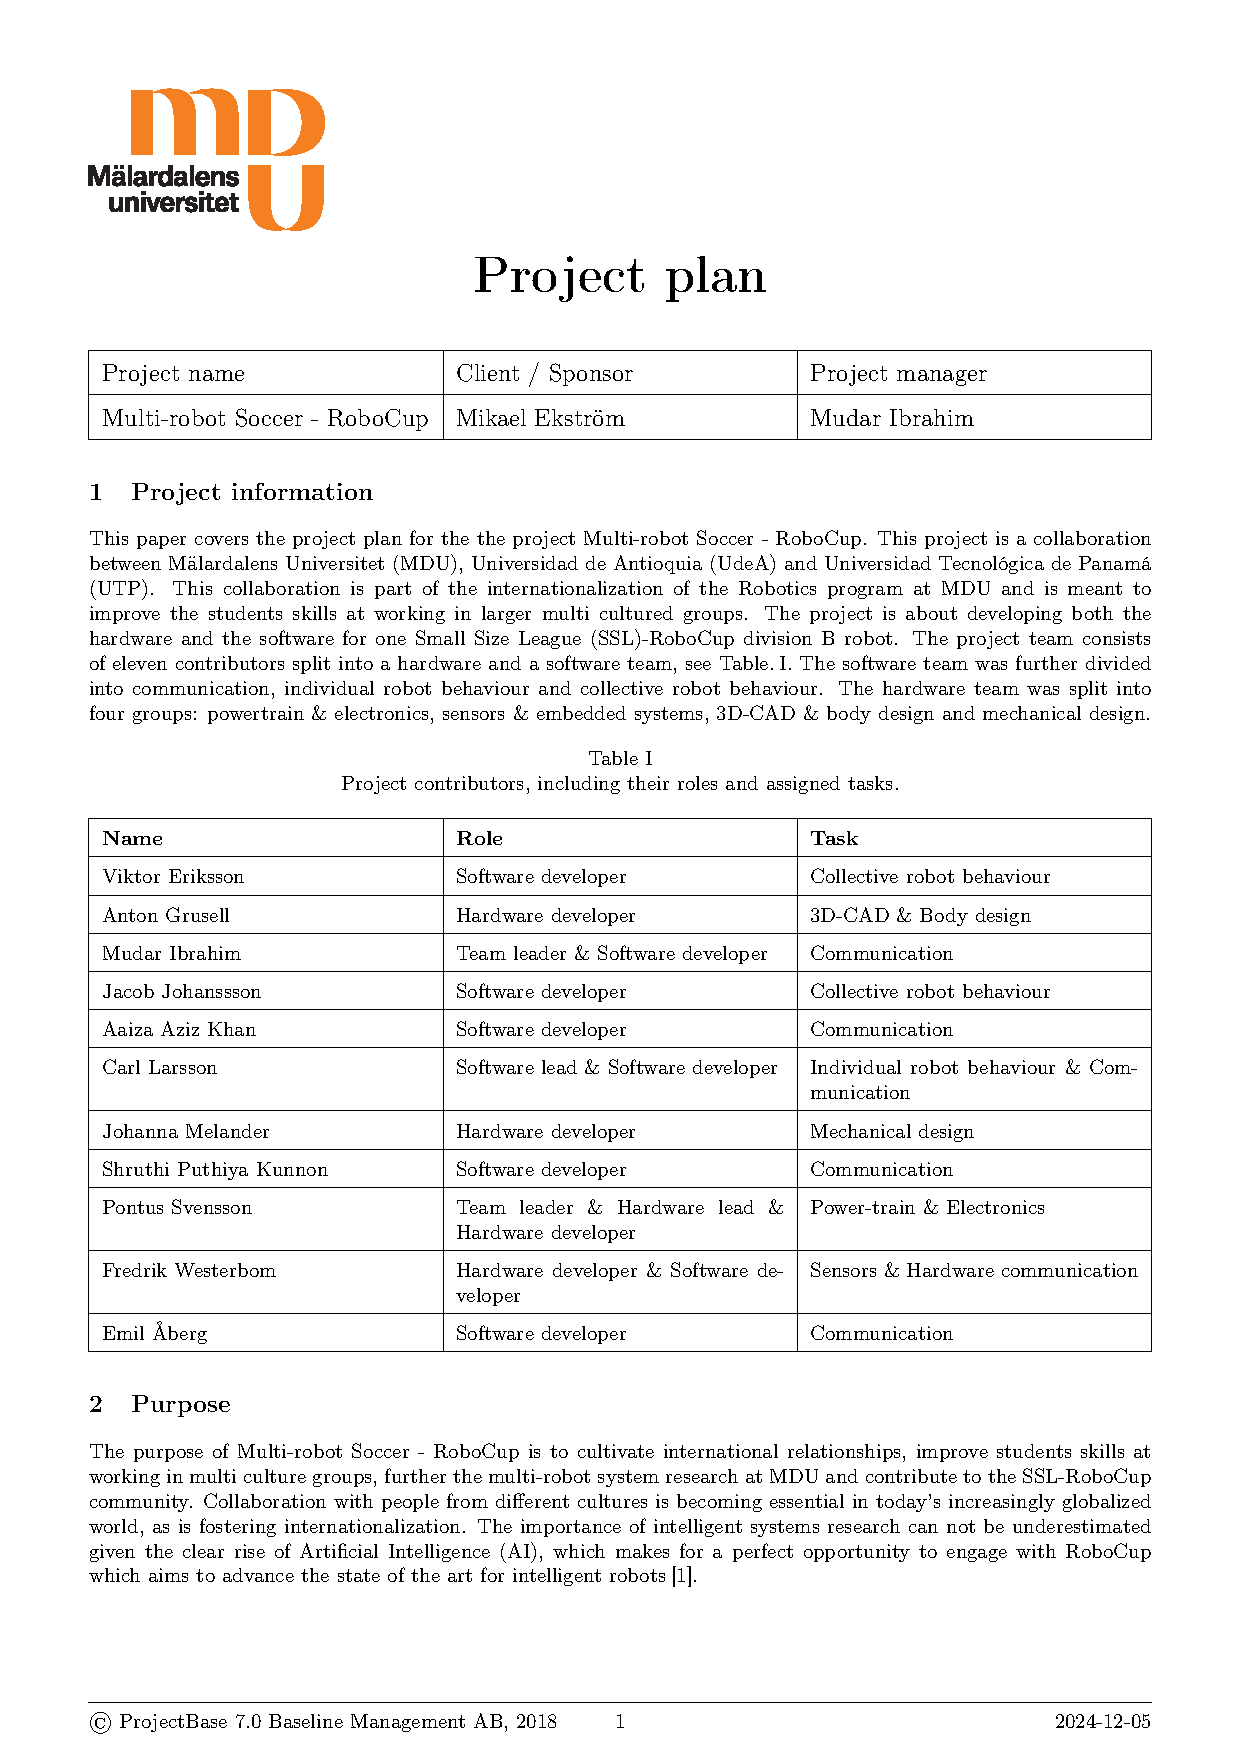
\includepdf[pages={1-}]{files/DVA490_474_PRO1.pdf}

%===============================================================================

%===============================================================================

\end{document}

%===============================================================================